\documentclass[a4paper, 11pt]{article}
\usepackage{amsmath}
\usepackage{graphicx}
\usepackage{geometry}
\usepackage{listings}
\usepackage{xcolor}
\usepackage{float}
\usepackage[fontset=ubuntu]{ctex}
\geometry{scale=0.8}
\linespread{1.5}
\usepackage{hyperref}

\lstset{
    %backgroundcolor=\color{red!50!green!50!blue!50},%代码块背景色为浅灰色
    rulesepcolor= \color{gray}, %代码块边框颜色
    breaklines=true,  %代码过长则换行
    numbers=left, %行号在左侧显示
    numberstyle= \small,%行号字体
    %keywordstyle= \color{blue},%关键字颜色
    commentstyle=\color{gray}, %注释颜色
    frame=shadowbox%用方框框住代码块
    }


\title{	
\normalfont \normalsize
\textsc{School of Data and Computer Science, Sun Yat-sen University} \\ [25pt] %textsc small capital letters
\rule{\textwidth}{0.5pt} \\[0.4cm] % Thin top horizontal rule
\huge  prolog  introduction \\ % The assignment title
\rule{\textwidth}{2pt} \\[0.5cm] % Thick bottom horizontal rule
\date{\normalsize October 1, 2020} 
}

\begin{document}
\maketitle
\tableofcontents
\newpage

\section{prolog introduction}
Prolog is a logic programming language. It was built on the theoretical basis of logic and was initially used in research fields such as natural language. Now it has been widely used in artificial intelligence research, it can be used to build expert systems, natural language understanding, intelligent knowledge bases, etc.

From now on, Prolog is mainly used in the domain of artificial intelligence and computer language. Different from general programming languages, prolog programs are based on the theory of predicate logic. The most basic way of writing is to establish the relationship between the object and the other, and then you can query the relationship between various objects by querying. The system will automatically match and backtrack to find out the answer to the question.

\section{prolog installation}
Download at https://www.swi-prolog.org/Download.html.According to different systems ,you should choose the one who is compatible.
\begin{figure}[ht]
\centering

\includegraphics[scale=0.6]{E05_2019096_Family/prolog introduction/pic/download.png}
\caption{ch}
\label{fig:label}
\end{figure}

\section{prolog grammar}
\subsection{Getting started}
Both Linux and Mac can start prolog by input "swipl" in the console, About Window system, you should search "prolog" and click the icon.  When you see ?-, you are successful.

\colorbox{pink}{\color{black} ?- }is common groups, eg:
\begin{figure}[ht]
\centering
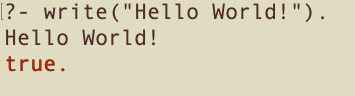
\includegraphics[scale=0.6]{E05_2019096_Family/prolog introduction/pic/code1.png}
\label{fig:label}
\end{figure}

All clause in prolog will be end with \colorbox{pink}{\color{black} . }. If you want to wrap, you can add\colorbox{pink}{\color{black} nl }in the  middle.
\begin{figure}[H]
\centering
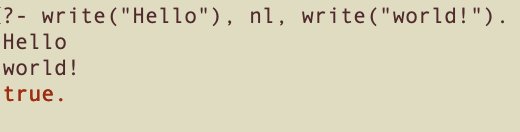
\includegraphics[scale=0.6]{E05_2019096_Family/prolog introduction/pic/code2.png}
\label{fig:label}
\end{figure}
If you want to exit prolog console, you can input \colorbox{pink}{\color{black} halt.}.

\subsection{Constant & variable}
The beginning of a lowercase string is a constant, and the beginning of an uppercase character is a variable,example:
\colorbox{pink}{\color{black} abc },this is a constant.
\colorbox{pink}{\color{black} Abc },this is a variable.
\begin{figure}[ht]
\centering
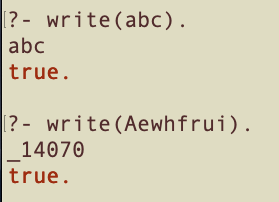
\includegraphics[scale=0.6]{E05_2019096_Family/prolog introduction/pic/code3.png}
\label{fig:label}
\end{figure}

\subsection{Relationship & attribute}
The relationship between two constants, we can use parentheses to specify , such as mike is jack's father,we can write as:\colorbox{pink}{\color{black} father(mike, jack). }. This is only a unilateral relationship, and the reverse is not necessarily true.\colorbox{pink}{\color{black} friend(x, y). }x is a friend of y, but y may be not his friend.If "friend" specify x and y are friends,we have to write again。\colorbox{pink}{\color{black} friend(x, y). friend(y, x). }

The two constants are expressed in parentheses, but if there is only one parameter, it means that the constant has this attribute.like \colorbox{pink}{\color{black} male(jack).},jack is male.

\subsection{rules}
Rules are the basis of reasoning. We can infer another conclusion from an existing conclusion based on the rules.
If x and y are friends, we need to repeat it twice:
\begin{figure}[ht]
\centering
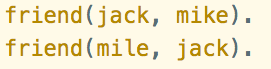
\includegraphics[scale=0.6]{E05_2019096_Family/prolog introduction/pic/code4.png}
\label{fig:label}
\end{figure}

Expressing by rules:

\begin{figure}[ht]
\centering
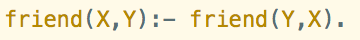
\includegraphics[scale=0.6]{E05_2019096_Family/prolog introduction/pic/code5.png}
\label{fig:label}
\end{figure}


\colorbox{pink}{\color{black} X,Y} are uppercase,they are variable,\colorbox{pink}{\color{black} :-}is reasoning,the same as\colorbox{pink}{\color{black} <-}. As long as the formula on the right side is true ,the formula on the left is true .If we augment with this rule , \colorbox{pink}{\color{black} friend(jack, mike). }can expressed as jack and mike are friends.
If a rule needs to apply multiple judgment conditions, like\colorbox{pink}{\color{black} X}is\colorbox{pink}{\color{black} Y}'s son:


\begin{figure}[H]
\centering

\includegraphics[scale=0.6]{E05_2019096_Family/prolog introduction/pic/code6.png}
\label{fig:label}
\end{figure}


\colorbox{pink}{\color{black} X}is\colorbox{pink}{\color{black} Y}'s son. Firstly, \colorbox{pink}{\color{black} X}is male,Secondly, \colorbox{pink}{\color{black} Y}may be\colorbox{pink}{\color{black} X}'s father or mother,there is a "or" relationship.In prolog,the \colorbox{pink}{\color{black} ,}and \colorbox{pink}{\color{black} ;}are "and" and "or" respectively .

If we want to set a rule is false,such as Unrequited love,love is \colorbox{pink}{\color{black} love(X,Y).}. And Unrequited love can be defined as:
\begin{figure}[H]
\centering

\includegraphics[scale=0.6]{E05_2019096_Family/prolog introduction/pic/code7.png}
\label{fig:label}
\end{figure}
If the rule following \colorbox{pink}{\color{black}$\backslash$+} is false,the whole rule can be matched.

\subsection{Compare}
There are two compare operations. \colorbox{pink}{\color{black} =} and \colorbox{pink}{\color{black} $\backslash$=}
\begin{lstlisting}[language={java}]
X = a, X = b.
X = a, Y = X.
\end{lstlisting}

The first one will return false. When one of the variables is not assigned and the other is a constant, the variables will be assigned a constant. And then the equal \colorbox{pink}{\color{black} =} will compare them.


The second one will return Y = a.When both are variables and one of them is already assigned, the unassigned variable will be assigned.

\begin{lstlisting}[language={java}]
X = a, X \= a.
\end{lstlisting}

Return false, 'X = a' will assign 'a' for X, and compare X and 'a'.

\subsection{Setof}
We have a knowledge base .

\begin{lstlisting}[language={java}]
age(peter, 7).
age(ann, 5).
age(pat, 8).
age(tom, 5).
age(ann, 5).

like(jack, ann).
age(X, 8) :- like(X, ann).
\end{lstlisting}

We can use \colorbox{pink}{\color{black} Setof} to get all the Children who has "age".(satisfy the age(X, Y).)
\begin{lstlisting}[language={prolog}]
?- setof(Child, age(Child, Age), Results).
Age = 5,
Results = [ann, tom] ;
Age = 7,
Results = [peter] ;
Age = 8,
Results = [jack, pat].
\end{lstlisting}

If any variables are used in "age(Child, Age)", which do not appear in the first argument(such as "Age"), "setof" will return a separate results for all possible.

We can do this in another way:
\begin{lstlisting}[language={prolog}]
?- setof(Age/Child, age(Child, Age), Results).
Results = [5/ann, 5/tom, 7/peter, 8/jack, 8/pat].
\end{lstlisting}

If we don't care about "Age" :
\begin{lstlisting}[language={prolog}]
?- setof(Child, Age^age(Child, Age), Results).
Results = [ann, jack, pat, peter, tom].
\end{lstlisting}

 Read: Find the all Children, such that the Child has an Age, and put the results in Results. 


\subsection{query}
Now, we should import the rules.
prepare a script \colorbox{pink}{\color{black} rules.pl},then import the script by \colorbox{pink}{\color{black} ?- [rules]}.(If you don’t know the path where your prolog reads the file by default,\colorbox{pink}{\color{black} ?- pwd}can help you.)

\begin{figure}[H]
\centering
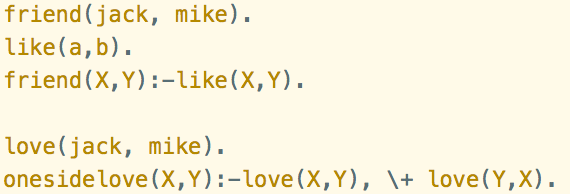
\includegraphics[scale=0.6]{E05_2019096_Family/prolog introduction/pic/code8.png}
\caption{rules.pl contain}
\end{figure}

\begin{figure}[H]
\centering
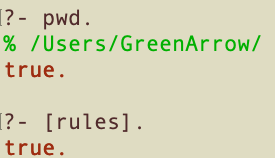
\includegraphics[scale=0.6]{E05_2019096_Family/prolog introduction/pic/code9.png}
\label{fig:label}
\caption{First check the default file path of prolog,Put rules.pl under this path,Use the [rules] command to import}
\end{figure}

Query:
\begin{figure}[H]
\centering
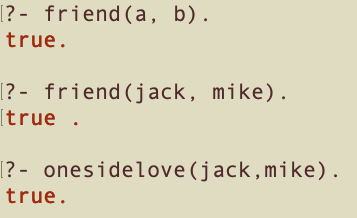
\includegraphics[scale=0.6]{E05_2019096_Family/prolog introduction/pic/code10.png}
\end{figure}

return\colorbox{pink}{\color{black} true.}means prolog find the matching one .We can also check what friends does Jack have:
\begin{figure}[H]
\centering
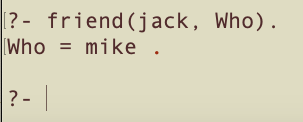
\includegraphics[scale=0.6]{E05_2019096_Family/prolog introduction/pic/code11.png}
\end{figure}

\section{Example}
\subsection{Factorial}
\begin{lstlisting}[language={java}]
factorial(N){
    if(N == 0 || N == 1) return 1;
    return factorial(N-1) * N;
}
\end{lstlisting}
First, we need to set the initial condition. When N == 1 || N == 0 ,return 1.
\begin{lstlisting}[language={java}]
factorial(1, 1).
factorial(0, 1).
\end{lstlisting}

When \colorbox{pink}{\color{black} N > 1}, \colorbox{pink}{\color{black} N = N - 1}, return \colorbox{pink}{\color{black} N * factorial(N-1)}. But here is factorial(N, Return), so we should calculate \colorbox{pink}{\color{black} factorial(N-1, Return1)} firstly, and then\colorbox{pink}{\color{black} Return = Return1 * N}.
\begin{lstlisting}[language={java}]
factorial(N,Ret) :-  N > 1, N1 is N - 1, factorial(N1, Ret1), Ret is N * Ret1.
\end{lstlisting}

\subsection{Fibonacci}
\begin{lstlisting}[language={java}]
fibonacci(N){
    if(N == 1 || N == 2) return 1;
    return fibonacci(N-1) + fibonacci(N-2);
}
\end{lstlisting}

Similarly, set initial condition:
\begin{lstlisting}[language={java}]
fibonacci(1, 1).
fibonacci(2, 1).
\end{lstlisting}

When \colorbox{pink}{\color{black} N > 2},  fibonacci(N-1) + fibonacci(N-2), but here is  fibonacci(N, return), N1 = N-1, N2 = N-2, calculate  fibonacci(N1, Return1) and fibonacci(N2, Return2) to get Return1 and Return2, Return = Return1 + Return2.

\begin{lstlisting}[language={prolog}]
fib(N,Ret) :- N > 2, N1 is N -1, N2 is N -2, fib(N1,Prv1), fib(N2,Prv2), Ret is Prv2 + Prv1.
\end{lstlisting}

If N > 2, then calculate fib(N1,Prv1), fib(N2,Prv2). Ret = Prv2 + Prv1 is the final return.

\subsection{Hanio}
\begin{lstlisting}[language={java}]
move(N, A, B, C){
    if(N==1){
       move A to C;
    }
    else
    {
        move(N-1,A,C,B);
        move A to C;
        move(N-1,B,A,C);
    }
}
\end{lstlisting}

If N == 1, we can move the object from A to C directly. But if N > 1, we have to move N-1 objects from A to B with the help of C firstly, then move the last one from A to C directly.Finaly, move N-1 objects from B to C with the help of A. 

Definition the problem:
\begin{lstlisting}[language={prolog}]
hanio(N) :- move(N, a, b, c).
\end{lstlisting}

We should move N objects from A to C.

In particular
\begin{lstlisting}[language={prolog}]
move(1,A,_,C):-inform(A,C).
\end{lstlisting}

When the numbers of objects just one,move from A to C directly.

\begin{lstlisting}[language={prolog}]
move(N,A,B,C):-N1 is N-1,move(N1,A,C,B),inform(A,C),move(N1,B,A,C).
\end{lstlisting}

Next, we move N-1 objects from A to B with the help of C (\colorbox{pink}{\color{black} move(N1,A,C,B)}), then move A to C.(\colorbox{pink}{\color{black} inform(A,C)}), finaly move n-1 objects from B to C with the help of A(\colorbox{pink}{\color{black} move(N1,B,A,C)}).

Definotion inform
\begin{lstlisting}[language={prolog}]
inform(Loc1,Loc2):-nl,write('from '),write(Loc1),write(' to '),write(Loc2).
\end{lstlisting}



%\clearpage
%\bibliography{E:/Papers/LiuLab}
%\bibliographystyle{apalike}
\end{document} 
%%% Local Variables:
%%% mode: latex
%%% TeX-master: t
%%% End:
\documentclass[a4paper, 11pt]{article}
\usepackage{amsmath}
\usepackage{graphicx}
\usepackage{geometry}
\usepackage{listings}
\geometry{scale=0.8}
\linespread{1.5}
\usepackage{hyperref}





%%% Local Variables:
%%% mode: latex
%%% TeX-master: t
%%% End:
